% !TeX spellcheck = cs_CZ
{\tikzset{external/prefix={tikz/MAI/}}
 \tikzset{external/figure name/.add={ch04_}{}}
%---------------------------------------------------------------------------------------------------
% file: Theory_of_Derivates.tex
%---------------------------------------------------------------------------------------------------
\chapter{Derivace funkce}\label{mai:IchapIV}
\minitoc

%============== Kapitola: Derivace funkce ==========================================================
  \section{Základní věty diferenciálního počtu}
    \subsection{Věta o největší (nejmenší) hodnotě funkce}
      V tomto článku uvedeme významné věty, zvané souhrně věty o \emph{střední hodnotě 
      diferenciálního počtu}, a dále pak ukázky jejich užití v matematické analýze.  Avšak dříve 
      než budeme tyto věty formulovat, uvedeme jedno důležité tvrzení, které sice bude mít v 
      dalších úvahách tohoto článku pomocnou úlohu, ale v teorii extrémů má i samostatný význam. 
      \cite[s.~186]{Brabec1989} 
      \begin{lemma}\label{MA1:lem_diff02}
        Nechť funkce $f:A\rightarrow\realset$ nabývá na množině $A$ své největší (nejmenší) hodnoty 
        na vnitřním bodě $c$ množiny $A$. Máli funkce $f$ v bodě $c$ derivaci, potom $f'(c)=0$.  
      \end{lemma}
      \begin{proof}
        Nechť např. $f(c)$ je největší hodnota funkce $f$ na množině $A$, takže $f(x)\leq f(c)$ pro $\forall x\in A$. Potom pro $x\in A, x<c$, je 
        $$\frac{f(x)-f(c)}{x-c}\geq 0$$
        a tedy
        $$f'_{-}(c)=\lim_{x\rightarrow c^-}\frac{f(x)-f(c)}{x-c}\geq0$$ 
        Dále pro $x\in A, x>c$, je
        $$\frac{f(x)-f(c)}{x-c}\leq 0$$ 
        a proto
        $$f'_{+}(c)=\lim_{x\rightarrow c^+}\frac{f(x)-f(c)}{x-c}\leq0$$
        Platí tedy
        $$f'_{+}(c)\leq f'_{-}(c)\geq f'_{-}(c).$$ 
        Avšak $f'_{+}(c)=f'_{-}(c)= f'(c)$. Odtud plyne $f'(c)=0$. 
      \end{proof}
      
    \subsection{Věty o střední hodnotě}
      \begin{lemma}\label{MA1:lem_diff03}
        \textbf{Rolleova věta}\footnote{Michel Rolle [Mišel Rol] (1652-1719) Francouzský matematik} Nechť funkce $f$ má tyto vlastnosti:
          \begin{enumerate}
            \item je spojitá na uzavřeném intervalu $\langle a,b\rangle$;
            \item má derivaci (vlastní či nevlastní) na otevřeném intervalu $(a,b)$;
            \item platí $f(a)=f(b)$.
          \end{enumerate}
        Potom v otevřeném intervalu $(a,b)$ existuje aspoň jeden bod $\xi$ takový, že $f'(\xi)=0$.   
      \end{lemma}
      \begin{proof}
        Protože je funkce $f$ je na uzavřeném intervalu $\langle a,b\rangle$ spojitá, nabývá v 
        tomto intervalu své největší hodnoty $M$,své nejmenší hodnoty $m$. Přitom ovšem platí:
        \begin{equation}\label{MA1:eq_diff02}
          m\leq f(x) \leq M, \qquad x\in\langle a,b\rangle.
        \end{equation}
        Nyní mohou nastat dva případy: 
        \begin{enumerate}
          \item funkce $f$ nabývá $M$ i $m$ právě v krajních bodech intervalu $\langle a,b\rangle$. Podle předpokladu 3 věty \ref{MA1:lem_diff03}
                však potom platí $f(a)=f(b)=m=M$. Vzhledem ke vztahu \ref{MA1:eq_diff02} odtud plyne, že funkce $f$ je konstantní na intervalu
                $\langle a,b\rangle$ a tedy $f'(x)=0$ dokonce v každém bodě $x\in(a,b)$
          \item Funkce $f$ nabývá apsoň jedné z hodnot $M$, $m$ v některém vnitřním bodě $\xi$ intervalu $\langle a,b\rangle$. Potom podle 
          věty \ref{MA1:lem_diff02} je $f'(\xi)=0$.         
        \end{enumerate}        
      \end{proof}
      \begin{note}
        Rolleova věta sama zaručuje jen existenci aspoň jednoho bodu $\xi\in(a,b)$, ve kterém je fe 
        $f'(\xi)=0$. Neumožňuje však ani určení tohoto bodu (nebo bodů), ani stanovení jejich počtu 
      \end{note}
      
      \begin{note}
        Na obr. \ref{MAI:fig_006} je ilustrován geometrický význam Rolleovy věty. Graf funkce na 
        tomto obrázku má v bodech $\xi_1$, $\xi_2$, v nichž je $f'(\xi_1)=f'(\xi_2)=0$ tečny 
        rovnoběžné s osou $x$. 
        \begin{figure}[ht!] %\ref{MAI:fig_004}
          \centering
          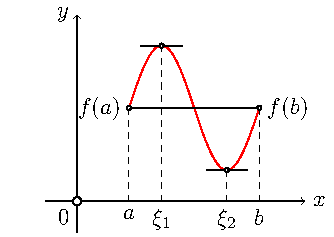
\includegraphics[width=0.7\linewidth]{MAI006.pdf}
          \caption{K výkladu Rolleovy věty}
          \label{MAI:fig_006}
        \end{figure}
      \end{note}
      
      Z Rolleovy věty plyne důležitá věta:
      
      \begin{lemma}\label{MA1:lem_diff04}
        (\textbf{Cauchyova věta}). Nechť funkce $f$ a $g$ mají tyto vlastnosti:
        \begin{enumerate}
          \item  Jsou spojité na uzavřeném intervalu $\langle a,b\rangle$,
          \item  v každém bodě $x\in(a,b)$ existuje derivace $f'(x)$ (vlastní či nevlastní) a vlastní derivace $g'(x)$,
          \item  $g'(x)\neq0$ na $(a,b)$
        \end{enumerate}
        Potom v otevřeném intervalu $(a,b)$ existuje aspoň jeden bod $\xi$, pro který platí
        \begin{equation}\label{MA1:eq_diff03}
          \frac{f(b)-f(a)}{g(b)-g(a)} = \frac{f'(\xi)}{g'(\xi)}.
        \end{equation} 
      \end{lemma} 
      
      \begin{proof}
        Poznamenejme především, že z předpokladu 3 $g'(x)\neq0$ pro $x\in(a,b)$ a z předpokladu 
        spojitosti funkce $g$ na uzavřeném intervalu $\langle a,b\rangle$ ihned vyplývá vztah 
        $g(b)- g(a)\neq 0$. Kdyby totiž bylo $g(b)=g(a)$, potom by podle \emph{Rolleovy věty} 
        \ref{MA1:lem_diff03} existoval aspoň jeden bod $\eta\in(a,b)$ takový že $g'(\eta)=0$. To 
        však by byl spor s předpokladem $g'(x)\neq0$ pro každý bod $x\in(a,b)$. Proto má smysl 
        podíl na levé straně rovnosti \ref{MA1:eq_diff03}
        
        K vlastnímu důkazu Cauchyovy věty zavedeme takovou pomocnou funkci $F$, aby splňovala podmínky Rolleovy věty. Definujme ji pro $x\in\langle a,b\rangle$ předpisem
        \begin{equation}\label{MA1:eq_diff04}
          F(x)=[f(b)-f(a)]\cdot[g(x)-g(a)]-[f(x)-f(a)]\cdot[g(b)-g(a)].
        \end{equation}
        Snadno ověříme, že tato funkce skutečně splňuje podmínky Rolleovy věty na intervalu $\langle a,b\rangle$:
        \begin{itemize}
          \item Je spojitá na intervalu $x\in\langle a,b\rangle$, což je důsledkem spojitosti  
                funkce $f$ a $g$ na intervalu $x\in\langle a,b\rangle$ ,
          \item má derivaci $F'$ na otevřeném intervalu $(a,b)$, což plyne z existence derivace  
                $f'$ a $g'$ funkce $f$ a $g$ na  intervalu $(a,b)$,
          \item $F(a)=F(b)=0$ 
        \end{itemize}
        Platí tedy i závěr Rolleovy věty pro funkci $F$, tj. na intervalu $(a,b)$ existuje aspoň 
        jeden bod $\xi$, pro který $F'(\xi)=0$. Zderivujeme-li funkci $F$, dostaneme (dosadíme-li 
        $x=\xi$): $$F'(\xi)=[f(b)-f(a)]g'(\xi)-f'(\xi)[g(b)-g(a)]=0$$ Odtud již plyne rovnost 
        \ref{MA1:eq_diff03}                  
      \end{proof}
      
      Významným zvláštním případem Cauchyovy věty je další věta, která se častěji používá.
      
      \begin{lemma}\label{MA1:lem_diff05}
        (\textbf{Lagrangeova věta})\footnote{Joseph Louis Lagrange [lagránž] (1736-1813), francouzský matematik}. Nechť funkce má tyto vlastnosti:
        \begin{itemize}
          \item Je spojitá na intervalu $\langle a,b\rangle$,
          \item má derivaci (vlastní či nevlastní) na otevřeném intervalu $(a,b)$. 
        \end{itemize} 
        Potom existuje v otevřeném intervalu $(a,b)$ aspoň jeden bod $\xi$, pro který platí 
        \begin{equation}\label{MA1:eq_diff05}
           \frac{f(b) - f(a)}{b - a} = f'(\xi),  
        \end{equation}  
        či-li
        \begin{equation}\label{MA1:eq_diff06}
           f(b) - f(a) = f'(\xi)(b-a),  
        \end{equation}           
      \end{lemma}
      
      \begin{proof}
        Tvrzení této věty je důsledkem tvrzení \emph{Cauchyovy věty}, a to pro případ $g(x)=x$. 
        Protože $g'(x)=1$ dokonce všude, jsou splněny všechny tři podmínky Cauchyovy věty. Proto 
        platí i závěr této věty, z něhož pro náš případ již plyne vzorec \ref{MA1:eq_diff05} a tedy 
        i vzorec \ref{MA1:eq_diff06}.  
      \end{proof}
      
      \begin{note}
        Podobně jako je Lagrangeova věta zvláštním případem věty Cauchyovy, je Rolleova věta zvláštním případem Lagrangeovy věty, a to přo případ, že $f(a)=f(b)$.
      \end{note}
      
      \begin{note}
        Lagrangeova věta se často nazývá \emph{větou o přírůstku funkce}, protože vzorcem \ref{MA1:eq_diff06} se vyjadřuje \emph{přírůstek funkce}, tj rozdíl $f(b)-f(a)$. 
        Všechny tři uvedené věty, tj. věta Rolleova, Cauchyova a Lagrangeova, se v literatuře nazývá souhrně \textbf{věty o střední hodnotě diferenciálního počtu}.
      \end{note}
      
      \begin{note}
        Na obr. ** je ilustrován geometrický význam Lagrangeovy věty. Podíl na levé straně rovnosti 
        \ref{MA1:eq_diff05}, tj. číslo $\frac{f(b) - f(a)}{b - a}$ je směrnice sečny $s$, spojující 
        body $A$, $B$ grafu funkce  $f$, které odpovídají krajním bodům intervalu $\langle 
        a,b\rangle$. Podle tvrzení Lagrangeovy věty existuje v otevřeném intervalu $(a,b)$ aspoň 
        jeden bod $\xi$ tak, že tečna grafu funkce $f$ v příslušném jeho bodě je rovnoběžná s 
        přímkou $s$.  
      \end{note}
      
      \begin{note}
        Z Lagrangeovy věty vyplývá toto tvrzení: Nechť funkce $f$ vyhovuje na intervalu $\langle a,b\rangle$ podmínkám Lagrangeovy věty a $x_1$, $x_2$ jsou dva libovolné různé body
        intervalu $\langle a,b\rangle$. Potom v otevřeném intervalu s krajnímy body $x_1$, $x_2$ existuje aspoň jeden bod $\xi$, pro který platí Lagrangeův vzorec:   
        \begin{align}
          f(x_2) - f(x_1)                  &= f'(\xi)(x_2-x_1) \label{MA1:eq_diff07} \\ 
          \frac{f(x_2) - f(x_1)}{x_2-x_1}  &= f'(\xi)          \label{MA1:eq_diff08}      
        \end{align}
        Potom bod $\xi$ lze vyjádřit takto:
        \begin{equation}\label{MA1:eq_diff09}  
          \xi = x_1 + \vartheta(x_2-x_1), \qquad \text{kde }\vartheta\in(0,1). 
        \end{equation}
        Označíme-li $x_2-x_1=h$, můžeme vzorec \ref{MA1:eq_diff07} napsat ve tvaru
        \begin{equation}
          f(x_1+h) - f(x_1)= f'(x_1 + \vartheta h)h, \qquad \text{kde }\vartheta\in(0,1). 
        \end{equation} 
      \end{note}       
          
    \subsection{Některé důsledky Lagrangeovy věty}
      Lagrangeova věta, má některé významné důsledky, které nyní uvedeme \cite[s.~189]{Brabec1989}:
      \begin{lemma}\label{MA1:lem_diff06} 
        Nechť funkce $f$ vyhovuje podmínkám Lagrangeovy věty a navíc nechť $f'(x)=0$ pro všechna 
        $x\in(a,b)$. Potom funkce $f$ je prostá na intervalu $\langle a,b \rangle$. 
      \end{lemma}
      \begin{proof}
        Necť $x_1, x_2$ jsou libovolné dva různé body intervalu $\langle a,b \rangle$. Potom podle 
        Lagrangeova vzorce \ref{MA1:eq_diff04} platí 
        \begin{equation}
          f(x_2) - f(x_1) = f'(\xi)(x_2-x_1) \neq0
        \end{equation}
        neboť $f'(\xi)\neq 0$ dle předpokladu.
      \end{proof}
      
      \begin{lemma}\label{MA1:lem_diff01}
        Funkce $f$ je konstantní na intervalu $(a,b)$, právě když má na tomto intervalu derivaci a platí $f'(x) = 0$ pro všechna $x\in(a,b)$. 
      \end{lemma}
      \begin{proof} Tedy
        \begin{itemize}
          \item Je-li funkce $f$ konstantní na intervalu $(a,b)$, pak je $f'(x) = 0$ pro všechna  
                $x\in(a,b)$, jak již víme.
          \item Nechť $f'(x) = 0$ pro všechna $x\in(a,b)$. Dokažme, že pro každé dva body $x_1, 
                x_2  \in(a,b)$, $x_1\neq x_2$, platí $f(x_1) = f(x_2)$. Z existence
                derivace vyplývá spojitost funkce a jsou tedy splněny podmínky Lagrangeovy věty na 
                každém intervalu $\langle x_1, x_2\rangle\subset(a,b)$. Podle vzorce 
                \ref{MA1:eq_diff04} tedy platí $f(x_2)-f(x_1)f'(\xi)(x_2-x_1)$, $\xi\in(x_1,x_2)$. 
                Protože podle předpokladu je $f'(x)=0$ pro $\forall x\in(a,b)$, platí $f(x_1) 
                -f(x_2)=0$, tj. $f(x_1)=f(x_2)$  
        \end{itemize}
      \end{proof}
      
} % tikzset
%---------------------------------------------------------------------------------------------------
\printbibliography[heading=subbibliography]
\addcontentsline{toc}{section}{Seznam literatury}